\documentclass[a4paper,14pt]{extarticle}

\usepackage{tikz,amsmath,graphicx,sistyle,xcolor}
\usepackage[a4paper,landscape,margin=-2mm]{geometry}

\usepackage{mathspec}

\setmainfont[
	Path = f/l/,
	BoldFont=lb.ttf,
	ItalicFont=li.ttf,
	BoldItalicFont=lbi.ttf
		]{l.ttf}
\setsansfont[
	Path = f/p/,
	BoldFont=pb.ttf,
	ItalicFont=pi.ttf,
	BoldItalicFont=pbi.ttf
		]{p.ttf}
		
\setmathfont(Digits)[Path = f/l/]{l.ttf}
\setmathfont(Latin)[Path = f/l/]{li.ttf}
\setmathfont(Greek)[Path = f/l/, Uppercase]{l.ttf}
\setmathfont(Greek)[Path = f/l/, Lowercase]{li.ttf}

\setmonofont[Path = f/p/]{p.ttf}

\begin{document}
\pagestyle{empty}

\def\hAt{-2}

\definecolor{cm}{RGB}{190,0,170}
\definecolor{half}{RGB}{45,190,80}
\definecolor{each}{RGB}{215,215,215}

\def\vertgrid{
	\foreach \y in {-6,...,4} {
		\draw[color=cm,very thick] (\hAt cm - 0.8 cm,\y cm)
			node[left]{\y}
			-- (\hAt cm - 0.4 cm,\y cm);
		\foreach \t in {1,...,9} {
			\draw[color=each,thick] (\hAt cm - 0.68 cm, \y cm + 0.1*\t cm)
				-- (\hAt cm - 0.52 cm, \y cm + 0.1*\t cm);
		};
		\draw[color=half,very thick]
			(\hAt cm - 0.71 cm, \y cm + 0.5 cm)
			-- (\hAt cm - 0.49 cm, \y cm + 0.5 cm);
	};
}

\definecolor{origtitle}{RGB}{0,136,214}

\newcommand\cert[5]
{\begin{center} \tikz{
	\draw (0,0) node{
		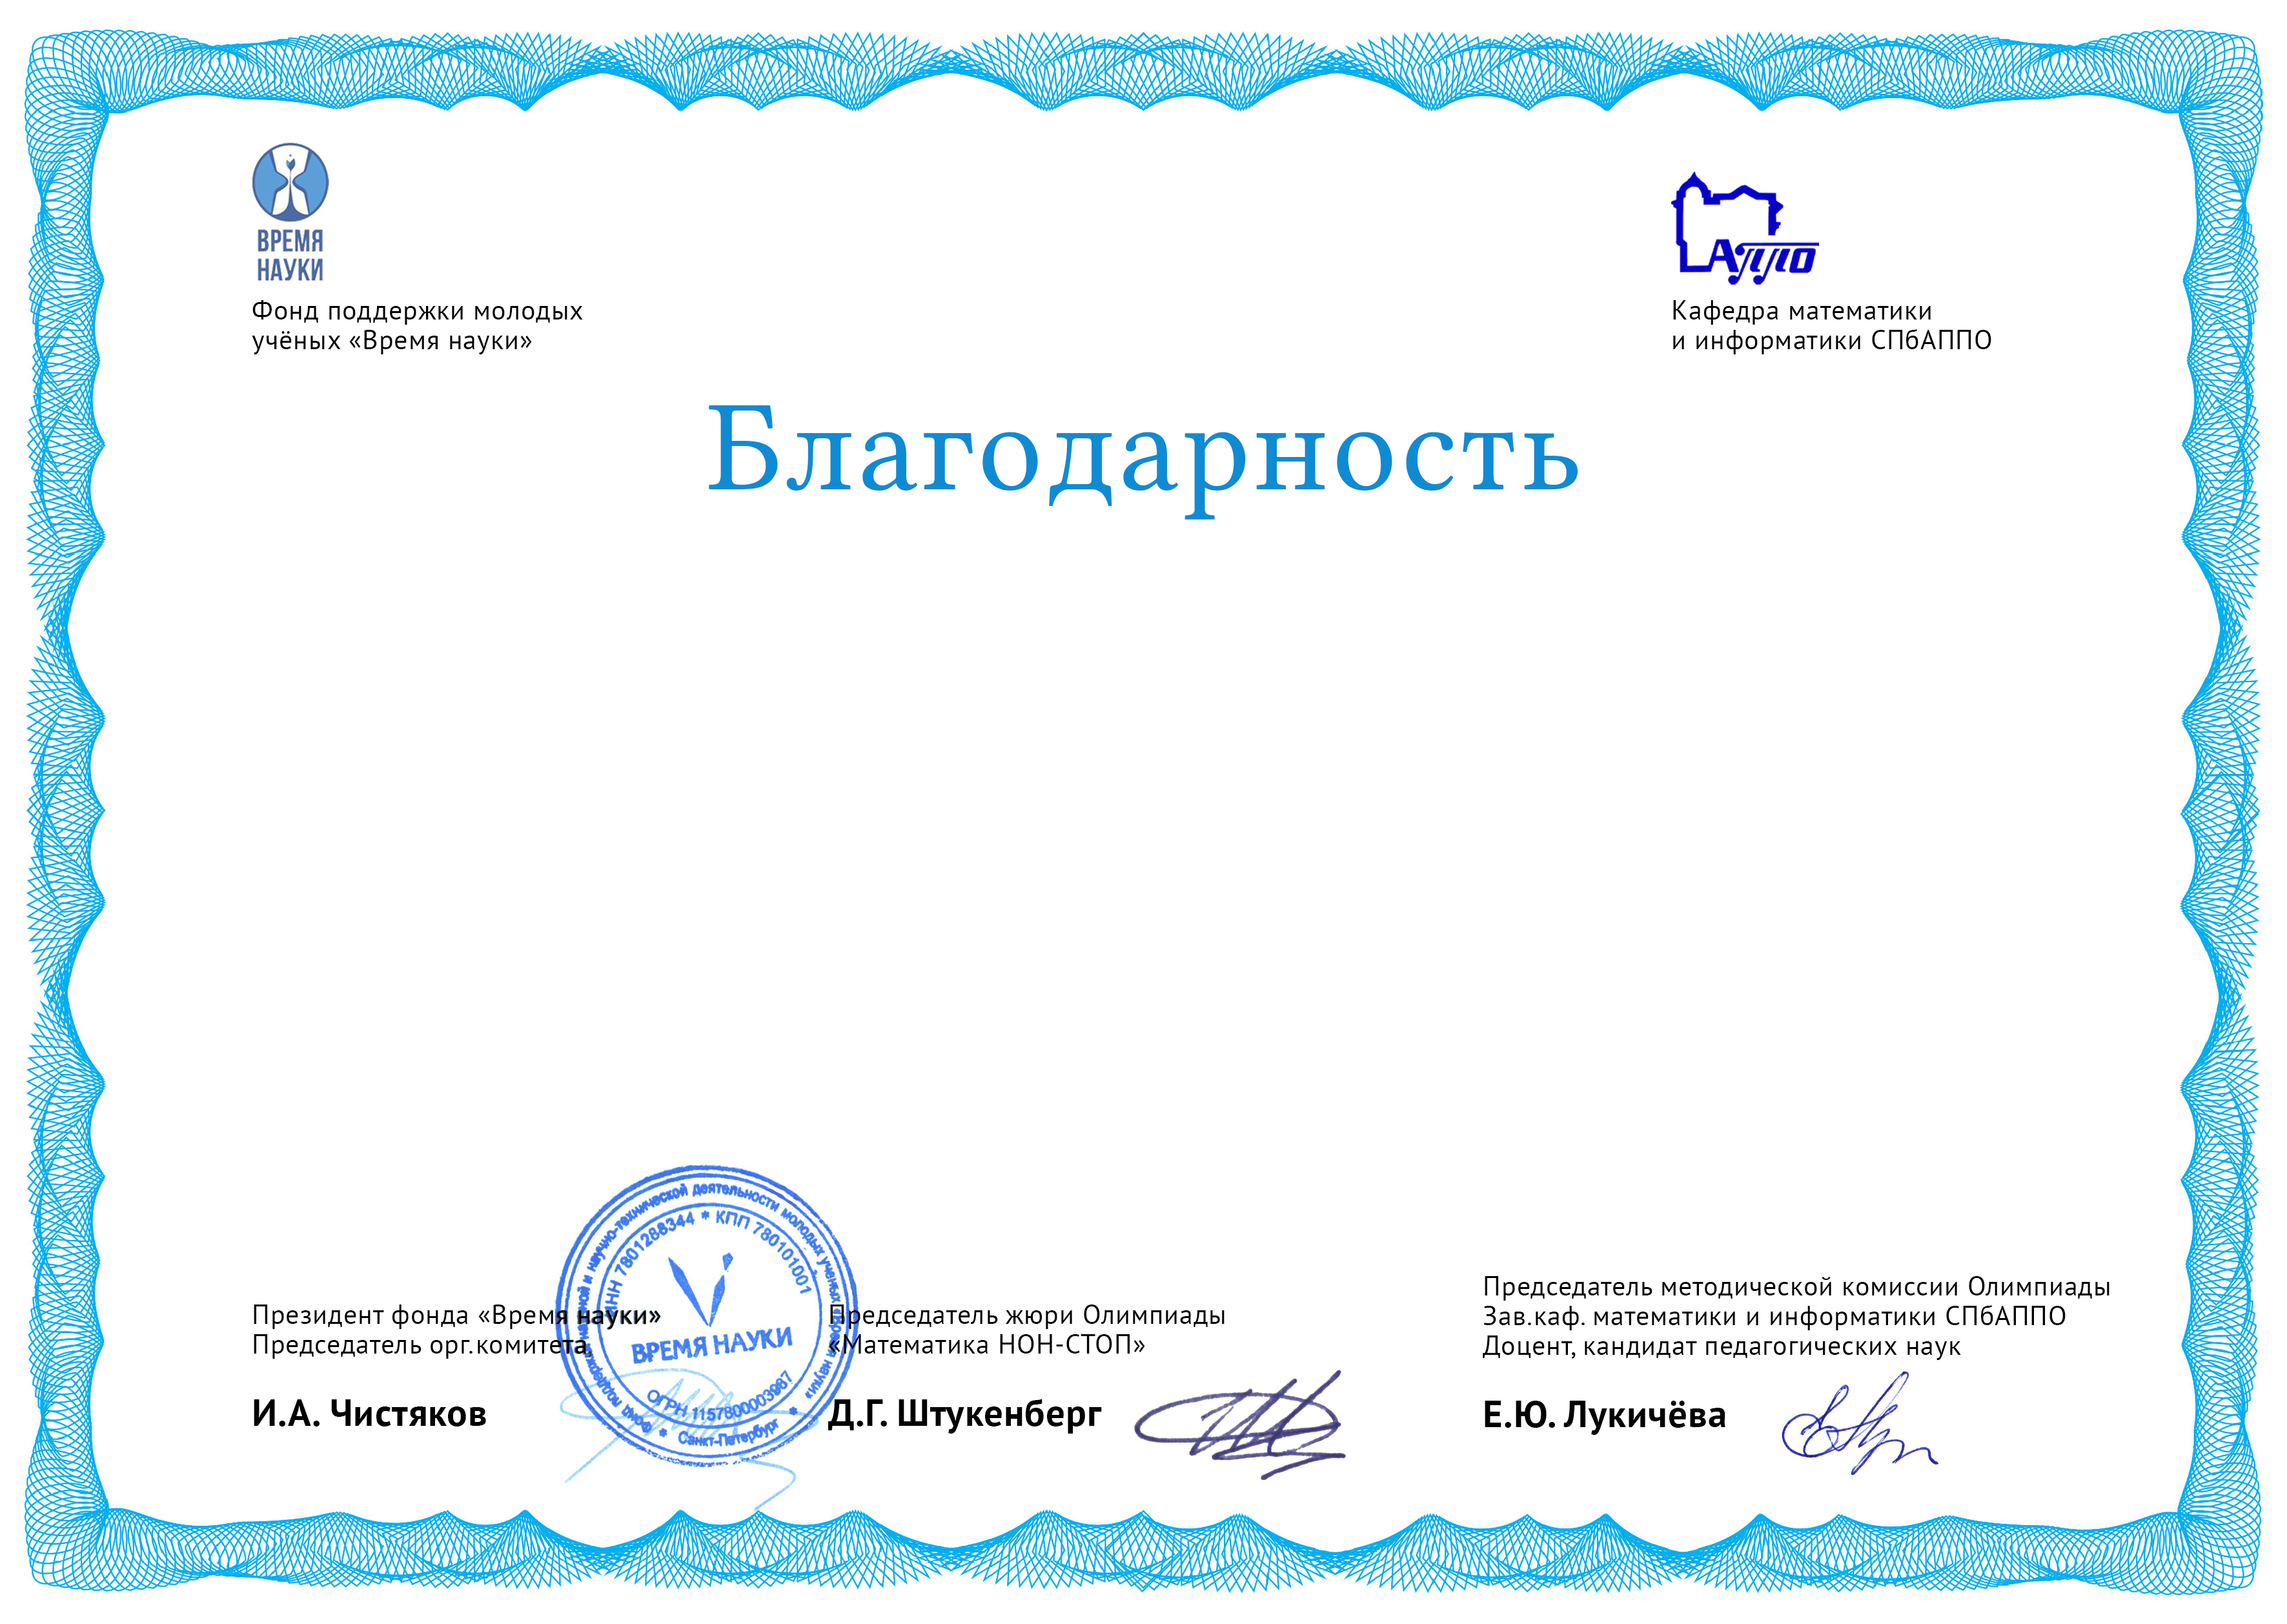
\includegraphics[width=29cm]{old/mns-maket-2020-grat}
	};
	\fill[white] (-7,3.5) rectangle (7,5.2);
	\draw (0, 4.45) node{\Huge\textcolor{origtitle}{Сертификат участника}};
	\draw (0,2.65) node{\Huge\bfseries #1};
	\draw (0,1.4) node{\large МКОУ «Сузунская СОШ №301 им.\,В.\,А.\,Левина», #2 класс};
	\draw (0,0.5) node{\large принимал#3 участие в олимпиаде};
	\draw (0,-0.4) node{\large {\bfseries «Математика НОН-СТОП — 2021»} с результатом};
	\draw (0,-1.55) node{\itshape\Large #4 баллов, #5 место};
	\draw (0,-2.7) node{\large Желаем Вам высоких наград};
	\draw (0,-3.6) node{\large и ждём в следующем году};
	\draw (0,-4.6) node{\Large\bfseries Успехов!};
%\vertgrid;
} \end{center} \vfill\eject}

\cert{Баталова Маргарита Михайловна}{5}{а}{0}{418}
\cert{Тарасенко Анастасия Романовна}{5}{а}{1}{395}
\cert{Муха Назар Александрович}{6}{}{3}{371}
\cert{Симоненко Матвей Петрович}{8}{}{0}{259}
\cert{Науршин Александр Евгеньевич}{8}{}{6}{200}
\cert{Блинова Анастасия Романовна}{8}{а}{3}{232}

\end{document}